The given equation of the curve can be rearranged as
\begin{align}
	xy-x-2y+1 &= 0 \\
        \label{eq:chapters/12/6/3/2/Eq1}
	\implies \vec{x}^\top\myvec{0 & \frac{1}{2} \\ \frac{1}{2} & 0}\vec{x} + \myvec{-1 & -2}\vec{x}+1 &= 0 
\end{align}
Thus, 
\begin{align}
	\vec{V} &= \myvec{ 0 & \frac{1}{2} \\ \frac{1}{2} & 0} \\
	\vec{u} &= -\myvec{\frac{1}{2} \\ 1} \\
	f &= 1 
\end{align}
$\because q_1 = 10$, the point of contact can be obtained as
\begin{align}
	 \vec{q} =\myvec{q_1 \\ q_2} = \myvec{10 \\ \frac{9}{8}}
\end{align}
  From \eqref{eq:conic_tangent_mq},
 the normal vector of the tangent to \eqref{eq:chapters/12/6/3/2/Eq1} is
\begin{align}
	\vec{n} = \myvec{1 \\ 64}
	\implies
	\vec{m} = \myvec{1 \\ \frac{-1}{64}}
\end{align}
The eigenvector matrix 
\begin{align}
	\myvec{\vec{p}_1 & \vec{p}_2} = \frac{1}{\sqrt{2}}\myvec{1 & 1 \\ 1 & -1}
\end{align}
which implies that  the conic is a $45\degree$ rotated hyperbola.
See \figref{fig:chapters/12/6/3/2/Fig1}.
\begin{figure}[H]
	\begin{center}
		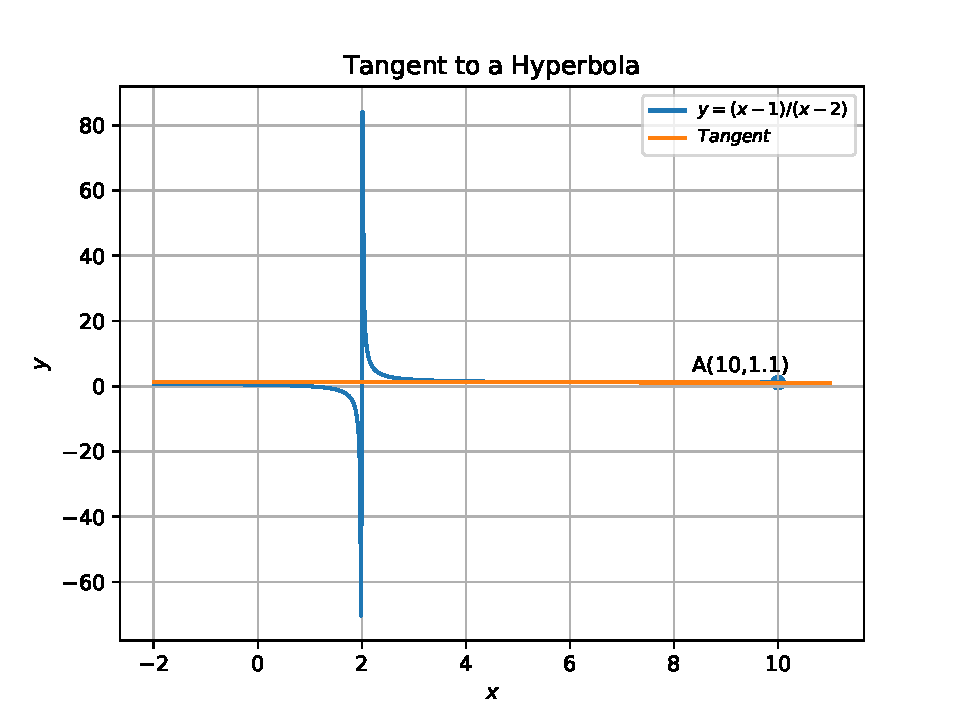
\includegraphics[width=0.75\columnwidth]{chapters/12/6/3/2/figs/problem2.pdf}
	\end{center}
\caption{}
\label{fig:chapters/12/6/3/2/Fig1}
\end{figure}
